
%% bare_conf.tex
%% V1.4b
%% 2015/08/26
%% by Michael Shell
%% See:
%% http://www.michaelshell.org/
%% for current contact information.
%%
%% This is a skeleton file demonstrating the use of IEEEtran.cls
%% (requires IEEEtran.cls version 1.8b or later) with an IEEE
%% conference paper.
%%
%% Support sites:
%% http://www.michaelshell.org/tex/ieeetran/
%% http://www.ctan.org/pkg/ieeetran
%% and
%% http://www.ieee.org/

%%*************************************************************************
%% Legal Notice:
%% This code is offered as-is without any warranty either expressed or
%% implied; without even the implied warranty of MERCHANTABILITY or
%% FITNESS FOR A PARTICULAR PURPOSE!
%% User assumes all risk.
%% In no event shall the IEEE or any contributor to this code be liable for
%% any damages or losses, including, but not limited to, incidental,
%% consequential, or any other damages, resulting from the use or misuse
%% of any information contained here.
%%
%% All comments are the opinions of their respective authors and are not
%% necessarily endorsed by the IEEE.
%%
%% This work is distributed under the LaTeX Project Public License (LPPL)
%% ( http://www.latex-project.org/ ) version 1.3, and may be freely used,
%% distributed and modified. A copy of the LPPL, version 1.3, is included
%% in the base LaTeX documentation of all distributions of LaTeX released
%% 2003/12/01 or later.
%% Retain all contribution notices and credits.
%% ** Modified files should be clearly indicated as such, including  **
%% ** renaming them and changing author support contact information. **
%%*************************************************************************


% *** Authors should verify (and, if needed, correct) their LaTeX system  ***
% *** with the testflow diagnostic prior to trusting their LaTeX platform ***
% *** with production work. The IEEE's font choices and paper sizes can   ***
% *** trigger bugs that do not appear when using other class files.       ***                          ***
% The testflow support page is at:
% http://www.michaelshell.org/tex/testflow/



\documentclass[conference]{IEEEtran}
% Some Computer Society conferences also require the compsoc mode option,
% but others use the standard conference format.
%
% If IEEEtran.cls has not been installed into the LaTeX system files,
% manually specify the path to it like:
% \documentclass[conference]{../sty/IEEEtran}





% Some very useful LaTeX packages include:
% (uncomment the ones you want to load)


% *** MISC UTILITY PACKAGES ***
%
%\usepackage{ifpdf}
% Heiko Oberdiek's ifpdf.sty is very useful if you need conditional
% compilation based on whether the output is pdf or dvi.
% usage:
% \ifpdf
%   % pdf code
% \else
%   % dvi code
% \fi
% The latest version of ifpdf.sty can be obtained from:
% http://www.ctan.org/pkg/ifpdf
% Also, note that IEEEtran.cls V1.7 and later provides a builtin
% \ifCLASSINFOpdf conditional that works the same way.
% When switching from latex to pdflatex and vice-versa, the compiler may
% have to be run twice to clear warning/error messages.






% *** CITATION PACKAGES ***
%
\usepackage{cite}
% cite.sty was written by Donald Arseneau
% V1.6 and later of IEEEtran pre-defines the format of the cite.sty package
% \cite{} output to follow that of the IEEE. Loading the cite package will
% result in citation numbers being automatically sorted and properly
% "compressed/ranged". e.g., [1], [9], [2], [7], [5], [6] without using
% cite.sty will become [1], [2], [5]--[7], [9] using cite.sty. cite.sty's
% \cite will automatically add leading space, if needed. Use cite.sty's
% noadjust option (cite.sty V3.8 and later) if you want to turn this off
% such as if a citation ever needs to be enclosed in parenthesis.
% cite.sty is already installed on most LaTeX systems. Be sure and use
% version 5.0 (2009-03-20) and later if using hyperref.sty.
% The latest version can be obtained at:
% http://www.ctan.org/pkg/cite
% The documentation is contained in the cite.sty file itself.






% *** GRAPHICS RELATED PACKAGES ***
%
\ifCLASSINFOpdf
  \usepackage[pdftex]{graphicx}
  % declare the path(s) where your graphic files are
  \graphicspath{{./pics/}}
  % and their extensions so you won't have to specify these with
  % every instance of \includegraphics
  \DeclareGraphicsExtensions{.pdf}
\else
  % or other class option (dvipsone, dvipdf, if not using dvips). graphicx
  % will default to the driver specified in the system graphics.cfg if no
  % driver is specified.
  % \usepackage[dvips]{graphicx}
  % declare the path(s) where your graphic files are
  % \graphicspath{{../eps/}}
  % and their extensions so you won't have to specify these with
  % every instance of \includegraphics
  % \DeclareGraphicsExtensions{.eps}
\fi
% graphicx was written by David Carlisle and Sebastian Rahtz. It is
% required if you want graphics, photos, etc. graphicx.sty is already
% installed on most LaTeX systems. The latest version and documentation
% can be obtained at:
% http://www.ctan.org/pkg/graphicx
% Another good source of documentation is "Using Imported Graphics in
% LaTeX2e" by Keith Reckdahl which can be found at:
% http://www.ctan.org/pkg/epslatex
%
% latex, and pdflatex in dvi mode, support graphics in encapsulated
% postscript (.eps) format. pdflatex in pdf mode supports graphics
% in .pdf, .jpeg, .png and .mps (metapost) formats. Users should ensure
% that all non-photo figures use a vector format (.eps, .pdf, .mps) and
% not a bitmapped formats (.jpeg, .png). The IEEE frowns on bitmapped formats
% which can result in "jaggedy"/blurry rendering of lines and letters as
% well as large increases in file sizes.
%
% You can find documentation about the pdfTeX application at:
% http://www.tug.org/applications/pdftex





% *** MATH PACKAGES ***
%
%\usepackage{amsmath}
% A popular package from the American Mathematical Society that provides
% many useful and powerful commands for dealing with mathematics.
%
% Note that the amsmath package sets \interdisplaylinepenalty to 10000
% thus preventing page breaks from occurring within multiline equations. Use:
%\interdisplaylinepenalty=2500
% after loading amsmath to restore such page breaks as IEEEtran.cls normally
% does. amsmath.sty is already installed on most LaTeX systems. The latest
% version and documentation can be obtained at:
% http://www.ctan.org/pkg/amsmath





% *** SPECIALIZED LIST PACKAGES ***
%
\usepackage{algorithmic}
\usepackage{algorithm}
\renewcommand{\algorithmicrequire}{\textbf{Input:}}
\renewcommand{\algorithmicensure}{\textbf{Output:}}
% algorithmic.sty was written by Peter Williams and Rogerio Brito.
% This package provides an algorithmic environment fo describing algorithms.
% You can use the algorithmic environment in-text or within a figure
% environment to provide for a floating algorithm. Do NOT use the algorithm
% floating environment provided by algorithm.sty (by the same authors) or
% algorithm2e.sty (by Christophe Fiorio) as the IEEE does not use dedicated
% algorithm float types and packages that provide these will not provide
% correct IEEE style captions. The latest version and documentation of
% algorithmic.sty can be obtained at:
% http://www.ctan.org/pkg/algorithms
% Also of interest may be the (relatively newer and more customizable)
% algorithmicx.sty package by Szasz Janos:
% http://www.ctan.org/pkg/algorithmicx




% *** ALIGNMENT PACKAGES ***
%
%\usepackage{array}
% Frank Mittelbach's and David Carlisle's array.sty patches and improves
% the standard LaTeX2e array and tabular environments to provide better
% appearance and additional user controls. As the default LaTeX2e table
% generation code is lacking to the point of almost being broken with
% respect to the quality of the end results, all users are strongly
% advised to use an enhanced (at the very least that provided by array.sty)
% set of table tools. array.sty is already installed on most systems. The
% latest version and documentation can be obtained at:
% http://www.ctan.org/pkg/array


% IEEEtran contains the IEEEeqnarray family of commands that can be used to
% generate multiline equations as well as matrices, tables, etc., of high
% quality.




% *** SUBFIGURE PACKAGES ***
%\ifCLASSOPTIONcompsoc
%  \usepackage[caption=false,font=normalsize,labelfont=sf,textfont=sf]{subfig}
%\else
%  \usepackage[caption=false,font=footnotesize]{subfig}
%\fi
% subfig.sty, written by Steven Douglas Cochran, is the modern replacement
% for subfigure.sty, the latter of which is no longer maintained and is
% incompatible with some LaTeX packages including fixltx2e. However,
% subfig.sty requires and automatically loads Axel Sommerfeldt's caption.sty
% which will override IEEEtran.cls' handling of captions and this will result
% in non-IEEE style figure/table captions. To prevent this problem, be sure
% and invoke subfig.sty's "caption=false" package option (available since
% subfig.sty version 1.3, 2005/06/28) as this is will preserve IEEEtran.cls
% handling of captions.
% Note that the Computer Society format requires a larger sans serif font
% than the serif footnote size font used in traditional IEEE formatting
% and thus the need to invoke different subfig.sty package options depending
% on whether compsoc mode has been enabled.
%
% The latest version and documentation of subfig.sty can be obtained at:
% http://www.ctan.org/pkg/subfig




% *** FLOAT PACKAGES ***
%
%\usepackage{fixltx2e}
% fixltx2e, the successor to the earlier fix2col.sty, was written by
% Frank Mittelbach and David Carlisle. This package corrects a few problems
% in the LaTeX2e kernel, the most notable of which is that in current
% LaTeX2e releases, the ordering of single and double column floats is not
% guaranteed to be preserved. Thus, an unpatched LaTeX2e can allow a
% single column figure to be placed prior to an earlier double column
% figure.
% Be aware that LaTeX2e kernels dated 2015 and later have fixltx2e.sty's
% corrections already built into the system in which case a warning will
% be issued if an attempt is made to load fixltx2e.sty as it is no longer
% needed.
% The latest version and documentation can be found at:
% http://www.ctan.org/pkg/fixltx2e


%\usepackage{stfloats}
% stfloats.sty was written by Sigitas Tolusis. This package gives LaTeX2e
% the ability to do double column floats at the bottom of the page as well
% as the top. (e.g., "\begin{figure*}[!b]" is not normally possible in
% LaTeX2e). It also provides a command:
%\fnbelowfloat
% to enable the placement of footnotes below bottom floats (the standard
% LaTeX2e kernel puts them above bottom floats). This is an invasive package
% which rewrites many portions of the LaTeX2e float routines. It may not work
% with other packages that modify the LaTeX2e float routines. The latest
% version and documentation can be obtained at:
% http://www.ctan.org/pkg/stfloats
% Do not use the stfloats baselinefloat ability as the IEEE does not allow
% \baselineskip to stretch. Authors submitting work to the IEEE should note
% that the IEEE rarely uses double column equations and that authors should try
% to avoid such use. Do not be tempted to use the cuted.sty or midfloat.sty
% packages (also by Sigitas Tolusis) as the IEEE does not format its papers in
% such ways.
% Do not attempt to use stfloats with fixltx2e as they are incompatible.
% Instead, use Morten Hogholm'a dblfloatfix which combines the features
% of both fixltx2e and stfloats:
%
% \usepackage{dblfloatfix}
% The latest version can be found at:
% http://www.ctan.org/pkg/dblfloatfix




% *** PDF, URL AND HYPERLINK PACKAGES ***
%
\usepackage{url}
% url.sty was written by Donald Arseneau. It provides better support for
% handling and breaking URLs. url.sty is already installed on most LaTeX
% systems. The latest version and documentation can be obtained at:
% http://www.ctan.org/pkg/url
% Basically, \url{my_url_here}.




% *** Do not adjust lengths that control margins, column widths, etc. ***
% *** Do not use packages that alter fonts (such as pslatex).         ***
% There should be no need to do such things with IEEEtran.cls V1.6 and later.
% (Unless specifically asked to do so by the journal or conference you plan
% to submit to, of course. )


% correct bad hyphenation here
\hyphenation{op-tical net-works semi-conduc-tor}

\renewcommand\IEEEkeywordsname{Keywords}
\begin{document}
%
% paper title
% Titles are generally capitalized except for words such as a, an, and, as,
% at, but, by, for, in, nor, of, on, or, the, to and up, which are usually
% not capitalized unless they are the first or last word of the title.
% Linebreaks \\ can be used within to get better formatting as desired.
% Do not put math or special symbols in the title.
%\title{Bare Demo of IEEEtran.cls\\ for IEEE Conferences}
\title{Implementation of TCP Large Receive Offload on Multi-core NPU Platform}

% author names and affiliations
% use a multiple column layout for up to three different
% affiliations
\author{\IEEEauthorblockN{Li Jie}
\IEEEauthorblockA{School of Computer\\
National University of\\Defense Technology\\
Changsha, China\\
Email: lijie13d@nudt.edu.cn}
\and
\IEEEauthorblockN{Chen Shuhui}
\IEEEauthorblockA{School of Computer\\
National University of\\Defense Technology\\
Changsha, China\\
Email: shchen@nudt.edu.cn}
\and
\IEEEauthorblockN{Su Jinshu}
\IEEEauthorblockA{School of Computer\\
National University of\\Defense Technology\\
Changsha, China\\
Email: sjs@nudt.edu.cn}}

% conference papers do not typically use \thanks and this command
% is locked out in conference mode. If really needed, such as for
% the acknowledgment of grants, issue a \IEEEoverridecommandlockouts
% after \documentclass

% for over three affiliations, or if they all won't fit within the width
% of the page, use this alternative format:
%
%\author{\IEEEauthorblockN{Michael Shell\IEEEauthorrefmark{1},
%Homer Simpson\IEEEauthorrefmark{2},
%James Kirk\IEEEauthorrefmark{3},
%Montgomery Scott\IEEEauthorrefmark{3} and
%Eldon Tyrell\IEEEauthorrefmark{4}}
%\IEEEauthorblockA{\IEEEauthorrefmark{1}School of Electrical and Computer Engineering\\
%Georgia Institute of Technology,
%Atlanta, Georgia 30332--0250\\ Email: see http://www.michaelshell.org/contact.html}
%\IEEEauthorblockA{\IEEEauthorrefmark{2}Twentieth Century Fox, Springfield, USA\\
%Email: homer@thesimpsons.com}
%\IEEEauthorblockA{\IEEEauthorrefmark{3}Starfleet Academy, San Francisco, California 96678-2391\\
%Telephone: (800) 555--1212, Fax: (888) 555--1212}
%\IEEEauthorblockA{\IEEEauthorrefmark{4}Tyrell Inc., 123 Replicant Street, Los Angeles, California 90210--4321}}




% use for special paper notices
%\IEEEspecialpapernotice{(Invited Paper)}




% make the title area
\maketitle

% As a general rule, do not put math, special symbols or citations
% in the abstract
\begin{abstract}
Nowadays, the ethernet is developing much faster than memory and CPU technologies, protocol processing has become the bottleneck of TCP performance on end systems. Modern NICs usually support offload techniques such as checksum offload and TCP Segmentation Offload(TSO), allowing the end system to offload some processing work onto the NIC hardware. In this paper, we propose an implementation of Large Receive Offload(LRO) on a multi-core NPU platform to improve TCP performance, particularly, we employ a so called active ACK mechanism to make very large packets(64KB) aggregation possible. We present experiment results to demonstrate the effectiveness of our proposal.
\end{abstract}

% no keywords
\begin{IEEEkeywords}
Multi-core NPU, TCP, LRO
\end{IEEEkeywords}
% For peer review papers, you can put extra information on the cover
% page as needed:
% \ifCLASSOPTIONpeerreview
% \begin{center} \bfseries EDICS Category: 3-BBND \end{center}
% \fi
%
% For peerreview papers, this IEEEtran command inserts a page break and
% creates the second title. It will be ignored for other modes.
\IEEEpeerreviewmaketitle



\section{Introduction}
% no \IEEEPARstart
%This demo file is intended to serve as a ``starter file''
%for IEEE conference papers produced under \LaTeX\ using
%IEEEtran.cls version 1.8b and later.
% You must have at least 2 lines in the paragraph with the drop letter
% (should never be an issue)
%I wish you the best of success.

%\hfill mds

%\hfill August 26, 2015
In the last few years, ethernet bandwidth has increased from 1Gbps to 100Gbps, while memory bandwidth from DDR2's 8533.33MBps\cite{wikiddr2} to DDR4's 19200MBps\cite{wikiddr4}, the top speed of processors settled around 4GHz and has not increased much since the year of 2005\cite{danowitz2012cpu}. This performance gap makes memory access and protocol processing become the bottleneck of TCP, instead of link capacity. The constantly increasing network bandwidth has caused a severe burden for CPU, optimizing TCP processing mechanism can mitigate this situation and improve TCP performance on end systems.

Traditional TCP acceleration techniques such as checksum optimization\cite{braden1989computing}\cite{mallory1990incremental}\cite{rijsinghani1994computation}\cite{kleinpaste1995software}, zero-copy\cite{chu1996zero} and interrupt coalescing\cite{dong2011optimizing} focused on the host side, protocol processing is still done by host CPU. TOE\cite{yeh2002introduction} can offload the entire TCP protocol processing workload and improve TCP performance dramatically, but its implementation is very complex and often causes security and compatibility issues\cite{mogul2003tcp}. TSO\cite{connery1999offload} optimizes TCP's data sending path by offloading the data segmentation and checksum calculation functions, the technique has become rather mature because of its simplicity. LRO\cite{grossman2005large} improves TCP performance by reducing the number of packet headers processed by CPU, but it works in the NIC driver layer and the packet aggregation job is still done by host CPU.

A multi-core Network Processing Unit(NPU) is an integrated circuit which has a feature set specifically targeted at the networking application domain, it usually has excellent packet processing capability for the following reasons:
\begin{enumerate}
\item More than a dozen hardware based, low-switching-overhead threads. The large number of hardware contexts enables software to more effectively leverage the inherent parallelism exhibited by packet processing applications.
\item Favorable I/O features. A multi-core NPU can import packets from network interface to memory with high throughput, moreover, its flexible dispatching component can distribute packets to different threads or cores according to application configurations and pipeline with the corresponding processing threads.
\item Well designed message passing mechanism among different threads. A multi-core NPU often employs cross-bar structure or SRAM as its message transfer medium, which makes thread synchronization efficient and elegant.
\end{enumerate}

Different TCP flows are weakly correlated and can be processed concurrently, this fact naturally leads to the idea of employing a multi-core NPU's excellent packet processing capability to accelerate TCP processing on an end system. In this paper, we propose to use multi-core NPU as NIC and implement LRO on it, our implementation reduces the number of packets processed by host network stack and the number of interrupts generated by NIC, eventually improves TCP performance on an end system. The experiment results demonstrate the effectiveness of our proposal. Further more, our implementation only involves the NIC hardware and driver layer, there is no difference between the multi-core NPU and a normal NIC from the kernel network stack's and user applications' angle, our implementation does not suffer TOE's compatibility and security problems.

\section{Related Work}
Large Receive Offload is a NIC driver layer technique for increasing TCP data receiving throughput, it works by aggregating multiple small data packets of the same flow into large but much fewer ones, the aggregated packets are then delivered to the kernel network stack for further processing, as shown in Figure \ref{driver_with_lro}.
\begin{figure}[!t]
\centering
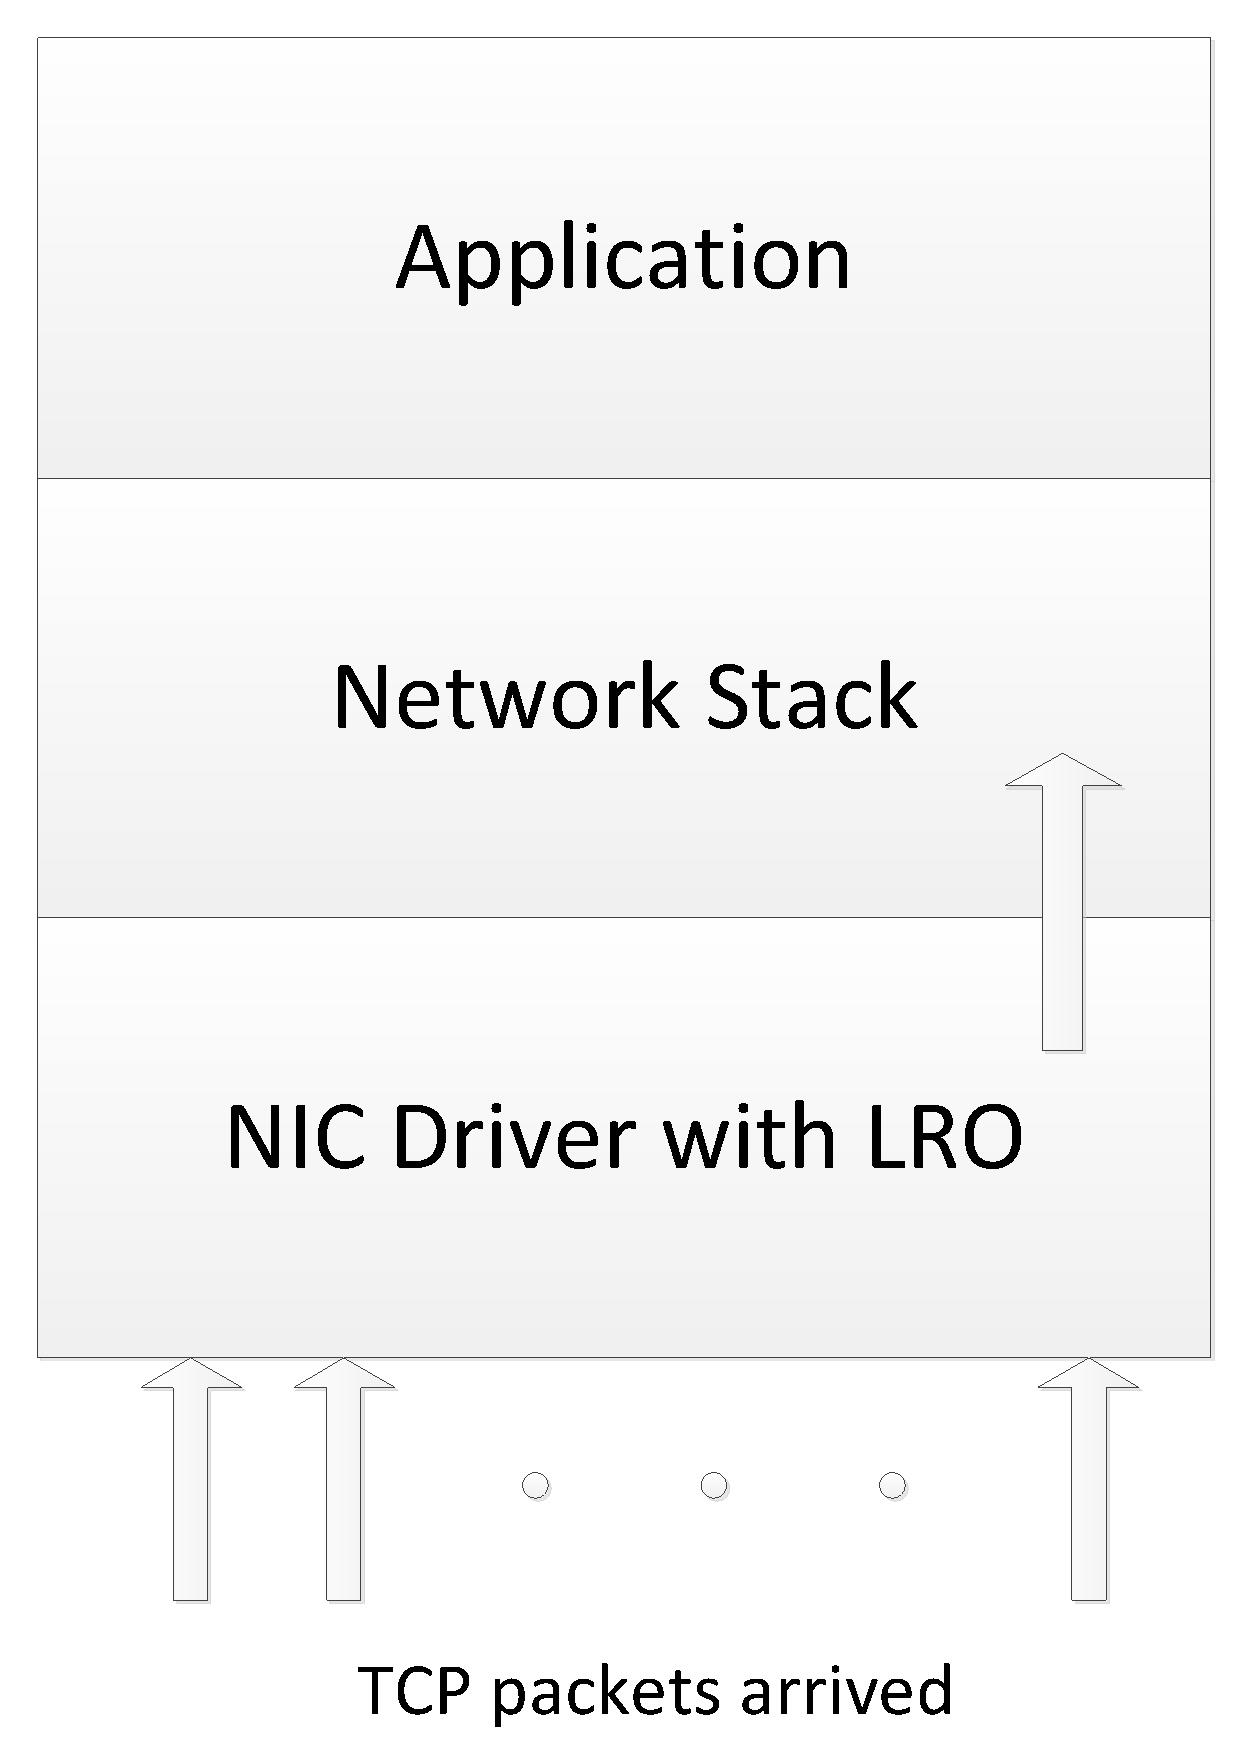
\includegraphics[width=1.5in]{nic_driver_with_lro}
% where an .eps filename suffix will be assumed under latex,
% and a .pdf suffix will be assumed for pdflatex; or what has been declared
% via \DeclareGraphicsExtensions.
\caption{NIC driver with LRO}
\label{driver_with_lro}
\end{figure}

LRO was first proposed by Grossman\cite{grossman2005large} and implemented in the NIC driver program for Neterion Xframe-II. When a packet arrives, driver program first decides whether to buffer the packet for aggregation, or discard the packet, or pass the packet directly to kernel network stack. Once the total data length of accumulated packets reaches a predefined threshold, driver program performs packets aggregation by setting appropriate values for the new packet's IP and TCP headers.

Themann\cite{theman2007lro} patched LRO into Linux operating system as a generic implementation, which enabled other developers to equip their NICs with LRO functionality through only a few code modifications.

Hatori\cite{hatori2008implementation} et al. implemented LRO in a Xen virtualized system on both physical and virtual interfaces, they achieved less CPU utilization and higher data receiving throughput. While Antichi\cite{antichi2013implementation} et al. implemented LRO on NETFPGA open hardware platform, their experiment results showed lower CPU utilization and packets drop rates, but the performance tests are conducted only on two concurrent TCP flows.
\section{System Architecture}
In our proposed scheme, we use multi-core NPU as NIC and implement LRO on it to accelerate TCP processing on the data receiving path. Packets reordering, packets aggregation and checksum verification(calculation) are done by the multi-core NPU, NIC driver program is responsible for forwarding the reconstructed big packet to the kernel network stack. Our system resides in the NIC hardware and driver layers, as shown in Figure \ref{nic_with_lro}.
\begin{figure}[!t]
\centering
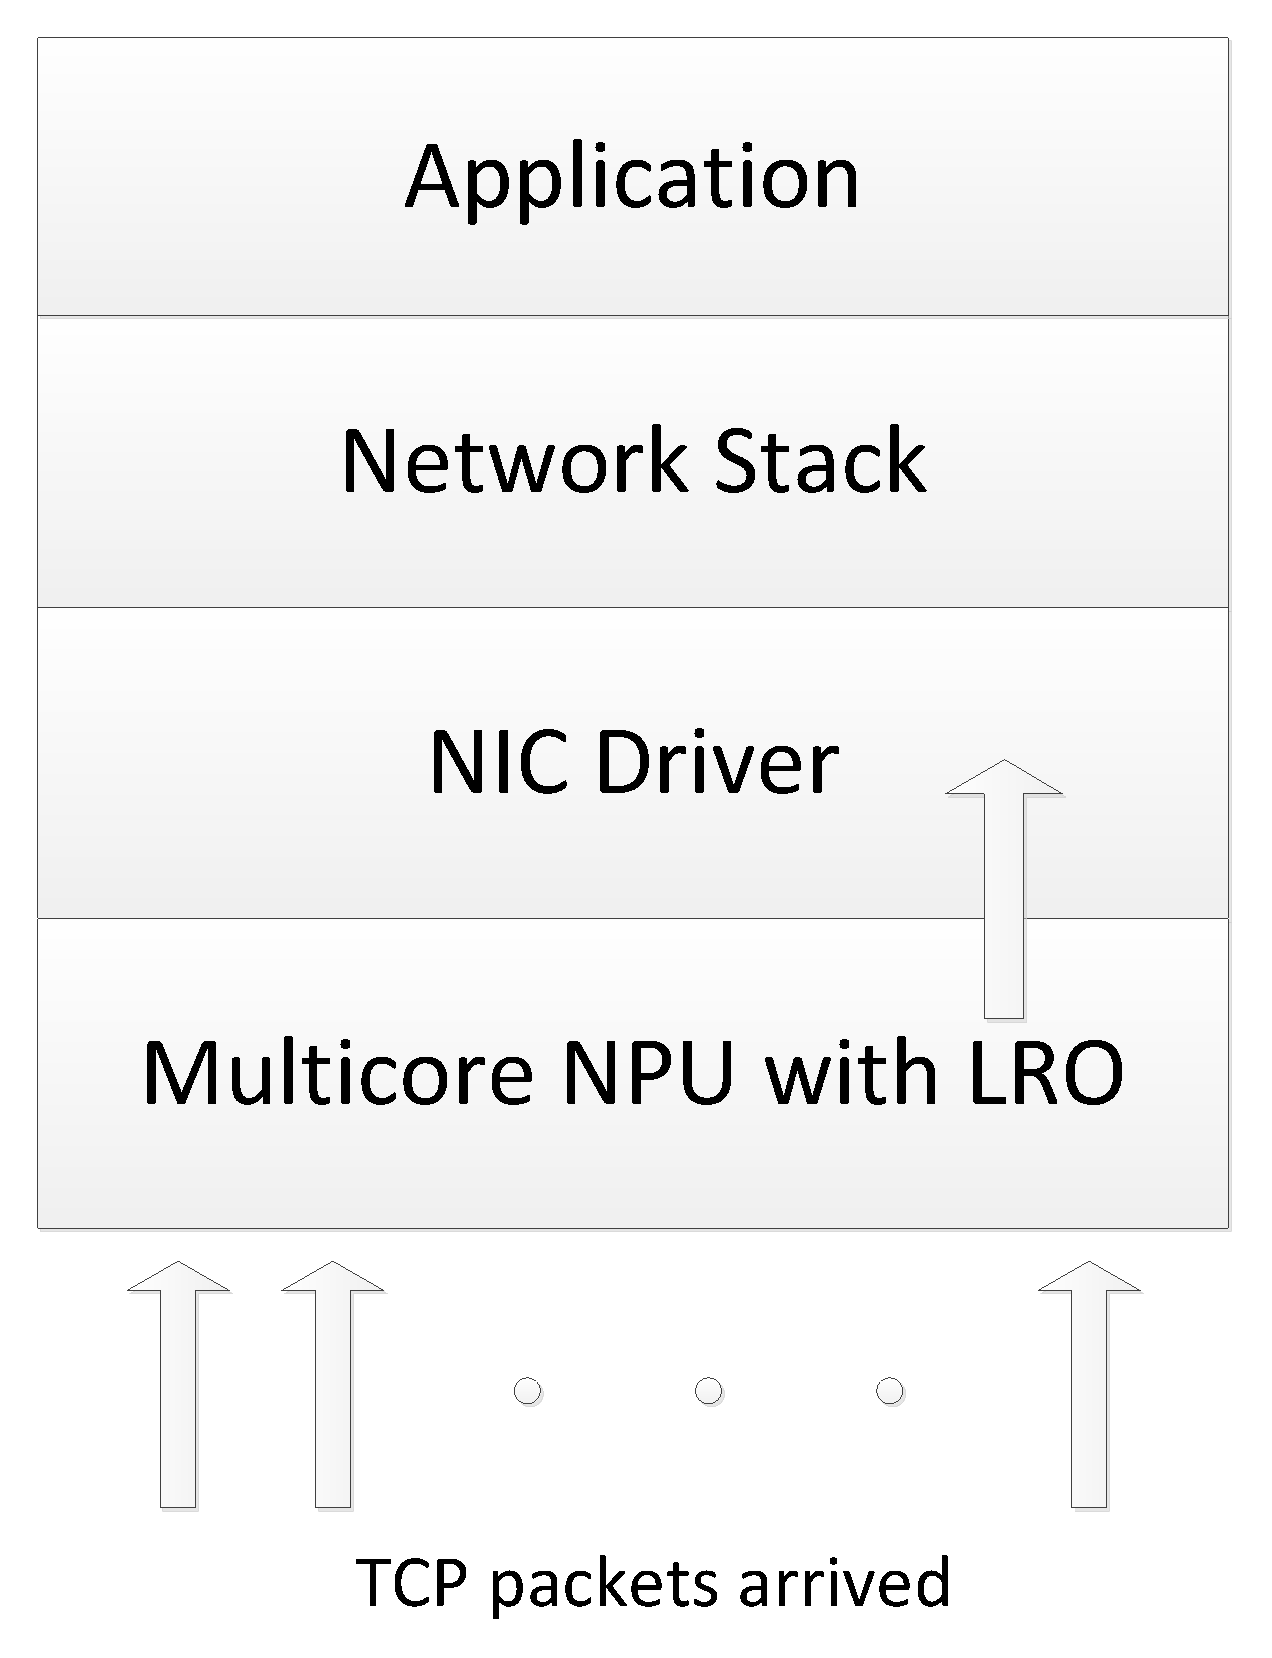
\includegraphics[width=1.5in]{nic_with_lro}
% where an .eps filename suffix will be assumed under latex,
% and a .pdf suffix will be assumed for pdflatex; or what has been declared
% via \DeclareGraphicsExtensions.
\caption{NIC with LRO}
\label{nic_with_lro}
\end{figure}

The multi-core NPU's numerous threads are divided into three categories: packet sending threads, packet receiving threads and a timeout checking thread(we will explain the reason of its existence in the next section).

The packet sending process is quite similar to a regular NIC, the receiving process of an ethernet packet, however, is much more complex. The multi-core NPU needs to check if a packet is suitable for LRO, handle out-of-order packets, check packet receiving timeout for a TCP flow, and reconstruct accumulated TCP data packets(we will describe these functionalities in more detail later). The packet receiving process sequence is shown in Figure \ref{packet receiving process sequence}: it starts by checking timeout messages, these messages are sent by a particular timeout checking thread, a timeout message indicates which TCP flow has paused(stopped) receiving new packets, and causes the multi-core NPU to aggregate buffered data packets of this flow. Then, the multi-core NPU checks for a newly arrived packet and runs a series of tests to see if the packet fits LRO requirements. If the packet passed those tests, it is buffered according to the TCP flow it belongs and reordered by its sequence number for further packets reconstruction; if it failed LRO tests, it will be forwarded directly to the NIC driver program(e.g. a UDP packet) or simply discarded(e.g. incorrect checksum).
\begin{figure}[!t]
\centering
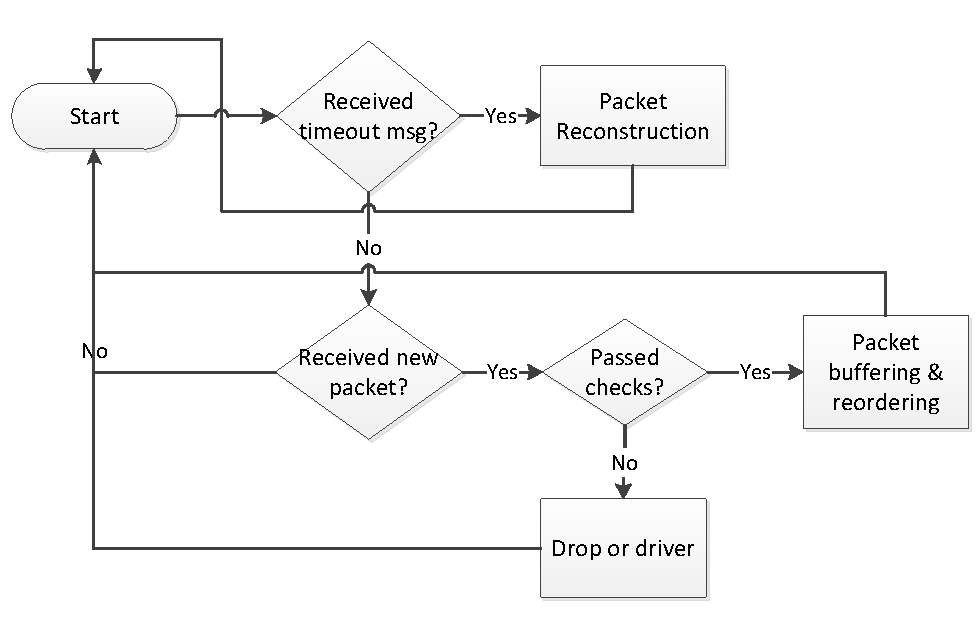
\includegraphics[width=3.0in]{packet_receiving_process_sequence}
% where an .eps filename suffix will be assumed under latex,
% and a .pdf suffix will be assumed for pdflatex; or what has been declared
% via \DeclareGraphicsExtensions.
\caption{Packet Receiving Process Sequence}
\label{packet receiving process sequence}
\end{figure}
Since the multi-core NPU has done nearly all the dirty work, the NIC driver program's job is rather simple and straight-forward, very like normal NIC driver programs except that: the driver program needs to pre-allocate consecutive pages for storing aggregated packet's data, and construct a correct skbuff data structure for it.
\section{System Functionalities}
\subsection{TCP Connection Management}
Our system employed two data structures for TCP connection management: ConnectionDescriptor and ConnectionTable.

ConnectionDescriptor is used to represent a TCP connection, it contains information including: the four-tuple which can uniquely identify a TCP connection; the number and total data length of buffered packets; and the maximum consecutive sequence number after packets reordering.

Each packet receiving thread of the multi-core NPU needs to maintain multiple TCP connections, i.e., multiple ConnectionDescriptors, thus a fast search mechanism is necessary. ConnectionTable is introduced to fulfill this requirement, it is designed as a hash table, and used for searching the corresponding ConnectionDescriptor when a TCP packet arrives. Our system utilizes the multi-core NPU's packet dispatch mechanism to distribute packets of the same connection to a fixed packet receiving thread. When a packet receiving thread receives a TCP packet, it calculates a hash value based on the packet's four-tuple, and looks for the corresponding ConnectionDescriptor via ConnectionTable. Each packet receiving thread maintains an independent ConnectionTable, so the search and update operations do not need to interact with other threads, synchronization overheads are naturally avoided.

Our system monitors TCP's three-way handshake sequence, when the multi-core NPU receives a SYN packet, it considers a TCP connection is being established. The corresponding packet receiving thread gets a free ConnectionDescriptor, initializes it with SYN packet's four-tuple information and adds it to the ConnectionTable.

Our system also monitors FIN packets to see if a connection is being tared down. When a packet receiving thread receives a FIN packet, it searches for the related ConnectionDescriptor, aggregates its buffered packets and generates an interrupt to make the driver program process this reconstructed packet. Then the ConnectionDescriptor is removed from ConnectionTable and marked as free for future use.

As with ConnectionTable, each packet receiving thread maintains its ConnectionDescriptors in an independant memory space to avoid thread synchronization operations.
\subsection{Packets Filtering}
Each packet receiving thread of the multi-core NPU runs a series of tests to see if a packet is appropriate for reordering and aggregation operations, packets which failed these tests are discarded or forwarded to the driver program, packets which passed these tests will be buffered on their corresponding ConnectionDescriptor for further processing. The detailed filter sequence is shown in Figure \ref{packets filtering}, note that we do not require packets' TCP sequence number to be consecutive.
\begin{figure}[!t]
\centering
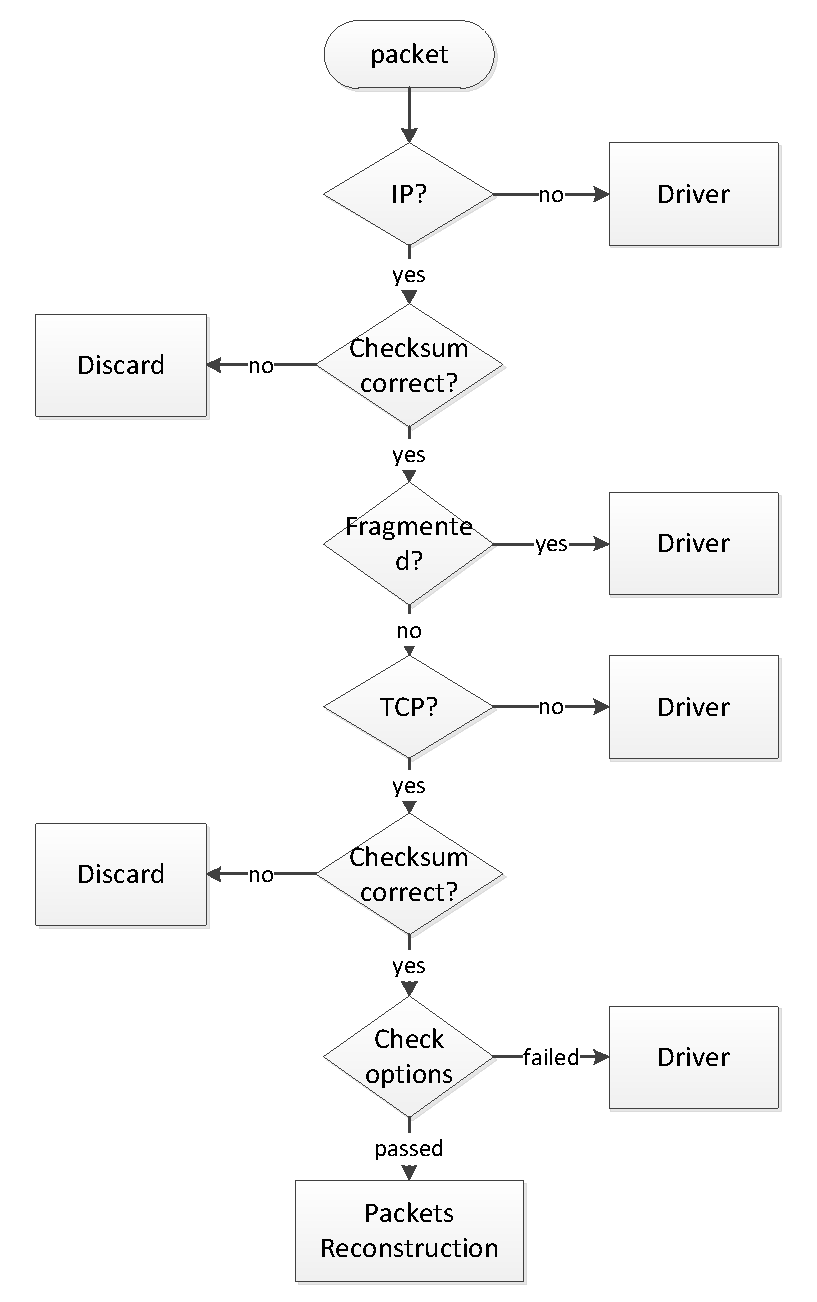
\includegraphics[width=2.0in]{filter_packets}
% where an .eps filename suffix will be assumed under latex,
% and a .pdf suffix will be assumed for pdflatex; or what has been declared
% via \DeclareGraphicsExtensions.
\caption{Packets Filtering}
\label{packets filtering}
\end{figure}
\subsection{Packets Reordering}
Each ConnectionDescriptor contains a list for buffering TCP data packets, multi-core NPU sorts packets by their TCP sequence number and stores them in increasing order. Pseudo code of our packets reordering algorithm is shown in Algorithm \ref{reorder_packet}.
\begin{algorithm}
\caption{ReorderPacket(pkt)}
\label{reorder_packet}
\begin{algorithmic}
\REQUIRE newly arrived TCP data packet
\STATE $desc \leftarrow SearchDescriptor(pkt)$
\IF{$desc.nextseq == pkt.seq$}
\STATE $Insert(pkt, desc)$
\STATE $UpdateNextSeq(desc)$
\ELSE \IF{$desc.nextseq > pkt.seq$}
    \STATE $Drop(pkt)$
    \ELSE \STATE $Insert(pkt, desc)$
    \ENDIF
\ENDIF
\end{algorithmic}
\end{algorithm}
The $Insert$ function adds a packet to its corresponding ConnectionDescriptor's packets list according to the TCP sequence number, or discards the packet if it has been transmitted before, as shown in Algorithm \ref{insert}.
\begin{algorithm}
\caption{Insert(pkt, desc)}
\label{insert}
\begin{algorithmic}
\REQUIRE TCP data packet and a connection descriptor
\FORALL{$p$ in $desc.pktlist$}
\IF{$p.seq == pkt.seq$}
\STATE $return$
\ELSE \IF{$p.seq > pkt.seq$}
    \STATE $insert\ pkt\ in\ front\ of\ p$
    \STATE $return$
    \ENDIF
\ENDIF
\ENDFOR
\end{algorithmic}
\end{algorithm}
Variable $nextseq$ records the maximum consecutive sequence number of buffered packets and infers consecutive data length of those packets. Time complexity of our packets reordering algorithm is $O(n)$, $n$ is number of buffered packets in a connection descriptor.
\subsection{Packets Reconstruction}
A packet receiving thread reconstructs buffered TCP data packets if one of the following three conditions holds:
\begin{enumerate}
\item consecutive payload length of the buffered packets has reached a predefined threshold
\item a FIN packet is received
\item one of its ConnectionDescriptors timed out for receiving packets
\end{enumerate}

The detailed processing sequence is shown in Figure \ref{tcp packets processing}.
\begin{figure}[!t]
\centering
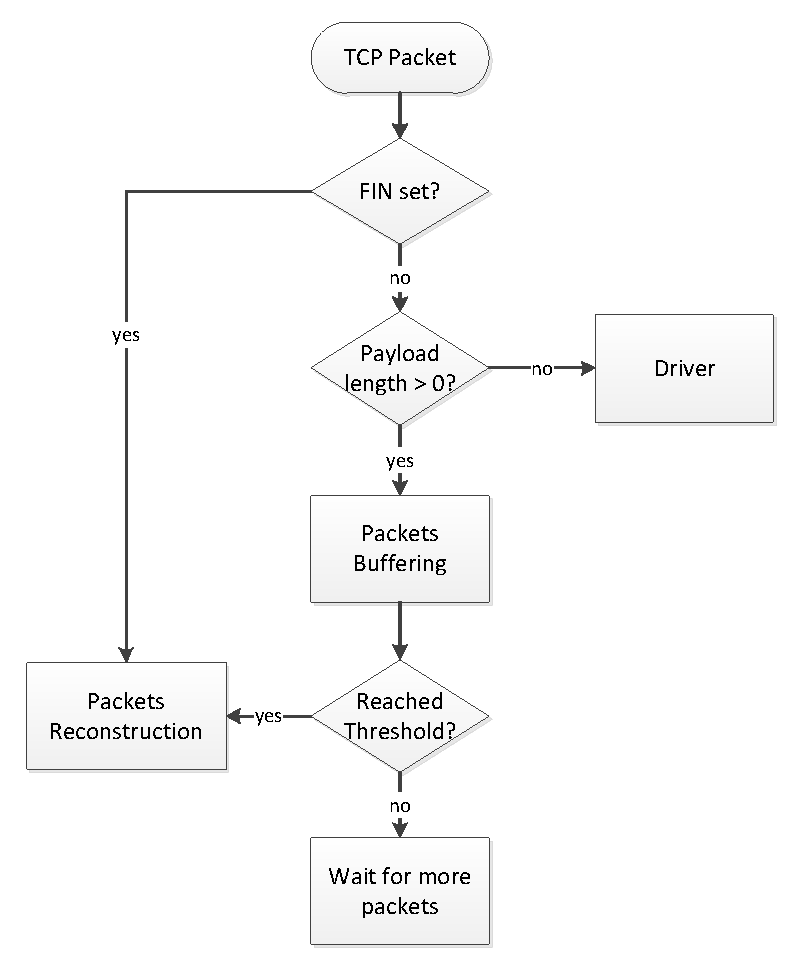
\includegraphics[width=2.0in]{tcp_packets_processing}
\caption{TCP Packets Processing}
\label{tcp packets processing}
\end{figure}
Packets reconstruction is done in two steps: (1) multi-core NPU modifies IP and TCP headers of the first packet, DMA the first packet's entire content(including headers) and the rest packets' payload data to host memory; (2) driver program constructs correct skbuff data structure for the aggregated packet and forward it to kernel network stack.
\subsection{Timeout Check for Packet Receiving}
A TCP connection can remain valid without any packet interactions for hours, the following situation explains the necessity of timeout check for packet receiving: multi-core NPU sets the threshold of buffered packets' data length to be 64KB, while the sending side only transmitted 8KB data and paused. Since the threshold is not reached and no FIN packet is received, the received data packets will be buffed in the multi-core NPU's memory permanently and will never reach to the data receiving host.

To solve this problem, each ConnectionDescriptor maintains two more variables for packet receiving timeout check: (1) $average\_interval$, which represents the average time interval of two adjacent packets; (2) $last\_arrival$, which records the last time ConnectionDescriptor received a packet. When a packet arrives, the packet receiving thread reads system time $current\_time$ and updates $average\_interval$ by the following formula: $average\_interval = (average\_interval + current\_time - last\_arrival) / 2$, $last\_arrival$ is updated by $current\_time$.

We used a specific thread of the multi-core NPU to execute the timeout checking task for every ConnectionDescriptor in our system, and named this thread as timeout checking thread. The timeout checking thread works in an infinite loop, it reads system's $current\_time$, a ConnectionDescriptor's $last\_arrival$ and calculates their difference, if the difference is larger than a hundred times of the ConnectionDescriptor's $average\_interval$, the corresponding TCP connection is considered as timed out. The timeout checking thread then sends a timeout message to the corresponding packet receiving thread, which performs packets reconstruction when received this message.
\section{Critical Improvement Techniques}
In this section, we will describe the critical techniques we employed to improve our system's performance.
\subsection{DMA Load Balance}
The multi-core NPU has an independent DMA engine which cooperates with hardware threads through message transmission. If a thread wants to transfer data between multi-core NPU and the host main memory, it sends a message which contains information including data source address, destination address and data length to the DMA engine; when the message is received, DMA engine executes the requested operation and sends a message back to the corresponding thread indicating whether the operation failed or succeeded.

A problem occurred when testing our system: we make the client test program to initiate multiple TCP connections to the server test program simultaneously and start data transmission after the connections are established, but we found that only a few connections can conduct data transmission normally while the rest connections' establishment failed due to timeout. The reason behind this phenomenon is that multi-core NPU's DMA engine buffers DMA request messages in a stack, when a few connections are established, they start data transmission immediately and overwhelm the DMA engine with request messages, other connections' SYN packets can not reach to the host kernel network stack and thus timed out.

To solve this problem, we utilized the timeout checking thread to add a DMA load balance functionality for the packet receiving threads: it maintains an individual DMA request message queue for each packet receiving thread, packet receiving threads now send DMA request messages to the timeout checking thread instead of the DMA engine, the timeout checking thread buffers these messages in their corresponding queues and chooses one message at a time in a Round-Robin fashion between the queues, the chosen message is then sent to the DMA engine. When the requested operation is done, DMA engine informs the corresponding packet receiving thread of the operation result by sending a message to it. Our DMA load balance mechanism only adds one more message exchange and two queue operations for each DMA request, it is highly efficient and simple for implementation.

\subsection{Active ACK Mechanism}
TCP sets a retransmission timer after sending data, if no corresponding ACK packet is received after the timer timed out, it retransmits data and performs congestion control by setting the data sending window size to 1 MSS(Maximum Segmentation Size). Consider the following situation: multi-core NPU sets data length threshold for packet aggregation larger than the amount of data the sending side can transmit before retransmission timer times out, it buffers received packets and waits for more to come, kernel network stack will not receive these packets thus no ACK is sent out, which eventually leads to data retransmission. What is worse, the retransmitted packets will be considered as redundant and discarded by the packet receiving threads, this makes data transmission unpracticable and violates our original purpose of TCP acceleration.

 An intuitive strategy for solving the afore-mentioned problem is to decrease multi-core NPU's data length threshold for packet aggregation and avoid retransmission timer timeout on the data sending side. But the underlying network and timeout value of the data sending side are constantly changing, which makes it difficult for the multi-core NPU to choose appropriate threshold values for each TCP connection. Decreasing threshold value also means more interrupts and more packet headers for the host kernel network stack to process, consequently the system performance suffers.

 TCP specifications tell us that duplicate ACKs are harmless, this fact leads to an alternative solution of our problem, we let the multi-core NPU mimic TCP's consecutive ACK mechanism: when a packet receiving thread receives a new packet, it performs packets reordering by inserting the packet to its corresponding ConnectionDescriptor's packets list, then it generates an ACK packet according to the ConnectionDescriptor's $nextseq$ value and sends the ACK to the data sending side. Particularly, we set the data receive window size to be 0xFFFF, which makes the sending side to transmit data faster.
\section{Implementation and Performance Evaluation}
We implemented our system using XLS416 produced by RMI, it has 16MB PCIe shared memory and 4GB DDR2 DRAM, the PCIe shared memory can be read/writen directly by host computer and XLS416, thus we used it for information sharing and store data structures such as packet descriptors, device state variables and miscellaneous counters. The 4GB DRAM is used by network interfaces for packet buffering and by hardware threads to maintain data structures such as ConnectionDescriptors and ConnectionTables.

XLS416's 16 hardware based threads are allocated as follows: 1 packet sending thread, 1 timeout checking thread, 13 packet receiving threads and the last one is reserved for system shell program. Our system optimizes TCP's data receiving path, thus only one thread is used for sending packets and as many as possible threads are used for receiving packets.

Most multi-core NPUs produced by RMI and other manufacturers are also equipped with XLS416's key hardware features, and only differentiates in specific configurations such as processing core frequency, DRAM and PCIe bandwidth. Data structures and algorithms we employed in our system can be easily implemented on other multi-core NPU platforms, resource allocation can also be done in a similar way, thus we conclude that our system design is highly compatible.

Our system focuses on optimizing TCP processing on the data receiving path, thus we chose TCP data receiving throughput as the performance evaluation criterion. We built two simple test programs including server side and client side: the client side first requests multiple TCP connections with the server, and starts data transmission after all the connections are established; server side records the time interval between connections' establishment and data transmission's completion, then calculates the data receiving throughput. Since our system buffers TCP data packets on the multi-core NPU, it is not suitable for delay-sensitive applications such as online games, instead, it is particularly suitable for applications with large blocks of data transmission such as ftp and samba servers. The client host is equipped with Intel Core i3 530 2.93GHz CPU, 4GB main memory and Intel 82599 NIC, the server host has the same hardware equipments except that it uses XLS416 as NIC, both hosts run Red Hat Enterprise Linux 6.4, a 10Gbps optical fiber is used to connect them back-to-back.

During the test, we set the number of TCP connections from 1 to 64 and calculate data receiving throughput respectively, the results are shown in Figure \ref{result}.

From Figure \ref{result} we can see that TCP data receiving throughput increases as the number of TCP connections increases when the latter is small, however, the growth slows down as the number of TCP connections becomes large and TCP data receiving throughput finally stabilizes around 4.75Gbps. The reason caused this phenomenon is the amount of packet receiving threads on XLS416 is fixed, when the number of TCP connections is small, XLS416 will dispatch packets to a subset of packet receiving threads and other threads are left idle, XLS416's computing power is not fully utilized; the situation changes as the number of TCP connections increases, packets will be evenly distributed to all threads and XLS416's computing power is exhausted, thus the maximum TCP data receiving throughput is achieved.
\begin{figure}[!t]
\centering
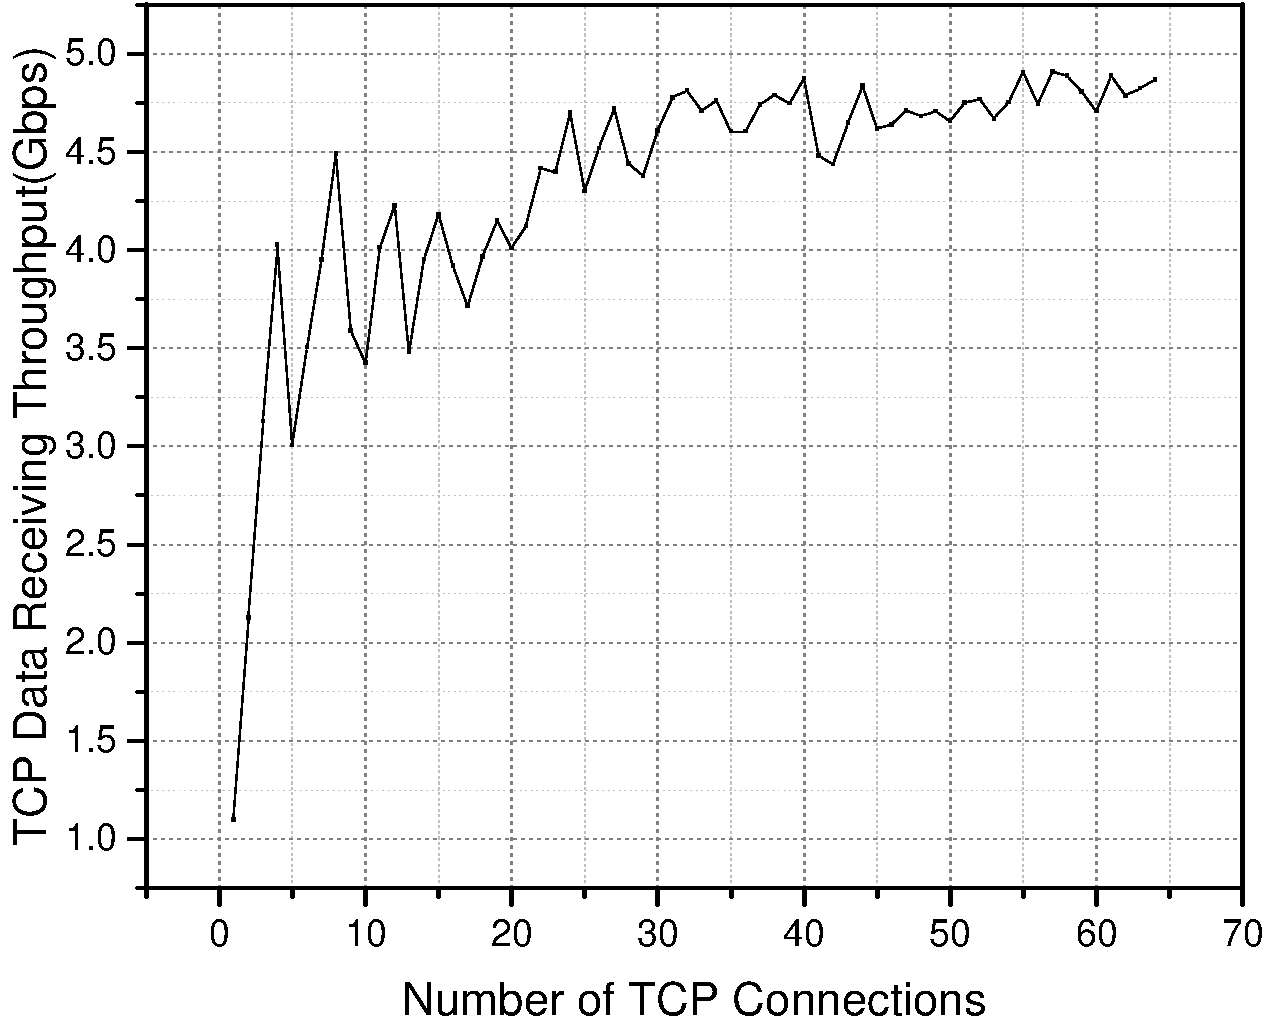
\includegraphics[width=2.5in]{oldresult}
\caption{TCP Data Receiving Throughput}
\label{result}
\end{figure}

As a comparison, we also implemented XLS416 as a normal NIC which does not aggregate TCP data packets and tested TCP data receiving throughput under the same hardware and software configurations, surprisingly, we found that TCP data receiving throughput is approximately 913.3Mbps and irrelevant to the number of TCP connections. The following factors lead to this huge performance gap:
\begin{enumerate}
\item when implemented as a regular NIC without LRO functionaliry, XLS416's computing power and storage space are nearly not used at all, multiple connections' packets are distributed to different threads, the threads then compete for the sole DMA engine to transfer packets' data to the host memory, this leads to a serial style access of the DMA engine and the overall TCP data receiving throughput is no different from a single connection situation. What is even worse, DMA engine restarts each time a request arrives and only transfers a small block of data(1500 bytes maximum), which results in a very poor performance. However, when XLS416 is implemented with LRO, a packet receiving thread requests DMA engine access for TCP data packets only when one of the three conditions which we stated in section IV is satisfied, most of the time, it buffers the packet, performs packets reordering job and waits for more packets, meanwhile the DMA engine can be used by another thread for data transmission. This leads to a pipelined style access of the DMA engine, thread synchronization overhead and DMA latency are hidden in the multiple packet receiving threads, DMA engine now transfers a large block of data(approximately 64KB) each time it is activated and a much better performance is achieved;
\item the number of packets processed by host CPU and interrupts generated by XLS416 become much more;
\item notice that the client's data sending speed affects the server's data receiving speed, when implemented with LRO functionality, XLS416 automatically generates ACK packets and causes the client side to send data faster, which in turn increases the server's data receiving throughput.
\end{enumerate}

To minimize the number of packets and interrupts processed by the host CPU, we chose Linux kernel data structure skbuff's storage upper bound(64KB) as the data length threshold for packets aggregation. We utilized XLS416's network accelerator for hardware checksum verification of incoming packets, the packets reordering and reconstruction algorithms used in our system are designed to be simple and efficient, which do not involve any packet data copy operation, XLS416's memory bandwidth should not be our system's performance bottleneck. On the other hand, XLS416, is actually a low-end product, which connects to the host computer through a PCI-e1.1$\times$4 bus, we tested its performance and achieved only 6Gbps data transmission throughput, thus we draw the conclusion that XLS416's PCI-e bandwidth is the performance bottleneck of our system.
% An example of a floating figure using the graphicx package.
% Note that \label must occur AFTER (or within) \caption.
% For figures, \caption should occur after the \includegraphics.
% Note that IEEEtran v1.7 and later has special internal code that
% is designed to preserve the operation of \label within \caption
% even when the captionsoff option is in effect. However, because
% of issues like this, it may be the safest practice to put all your
% \label just after \caption rather than within \caption{}.
%
% Reminder: the "draftcls" or "draftclsnofoot", not "draft", class
% option should be used if it is desired that the figures are to be
% displayed while in draft mode.
%
%\begin{figure}[!t]
%\centering
%\includegraphics[width=2.5in]{myfigure}
% where an .eps filename suffix will be assumed under latex,
% and a .pdf suffix will be assumed for pdflatex; or what has been declared
% via \DeclareGraphicsExtensions.
%\caption{Simulation results for the network.}
%\label{fig_sim}
%\end{figure}

% Note that the IEEE typically puts floats only at the top, even when this
% results in a large percentage of a column being occupied by floats.


% An example of a double column floating figure using two subfigures.
% (The subfig.sty package must be loaded for this to work.)
% The subfigure \label commands are set within each subfloat command,
% and the \label for the overall figure must come after \caption.
% \hfil is used as a separator to get equal spacing.
% Watch out that the combined width of all the subfigures on a
% line do not exceed the text width or a line break will occur.
%
%\begin{figure*}[!t]
%\centering
%\subfloat[Case I]{\includegraphics[width=2.5in]{box}%
%\label{fig_first_case}}
%\hfil
%\subfloat[Case II]{\includegraphics[width=2.5in]{box}%
%\label{fig_second_case}}
%\caption{Simulation results for the network.}
%\label{fig_sim}
%\end{figure*}
%
% Note that often IEEE papers with subfigures do not employ subfigure
% captions (using the optional argument to \subfloat[]), but instead will
% reference/describe all of them (a), (b), etc., within the main caption.
% Be aware that for subfig.sty to generate the (a), (b), etc., subfigure
% labels, the optional argument to \subfloat must be present. If a
% subcaption is not desired, just leave its contents blank,
% e.g., \subfloat[].


% An example of a floating table. Note that, for IEEE style tables, the
% \caption command should come BEFORE the table and, given that table
% captions serve much like titles, are usually capitalized except for words
% such as a, an, and, as, at, but, by, for, in, nor, of, on, or, the, to
% and up, which are usually not capitalized unless they are the first or
% last word of the caption. Table text will default to \footnotesize as
% the IEEE normally uses this smaller font for tables.
% The \label must come after \caption as always.
%
%\begin{table}[!t]
%% increase table row spacing, adjust to taste
%\renewcommand{\arraystretch}{1.3}
% if using array.sty, it might be a good idea to tweak the value of
% \extrarowheight as needed to properly center the text within the cells
%\caption{An Example of a Table}
%\label{table_example}
%\centering
%% Some packages, such as MDW tools, offer better commands for making tables
%% than the plain LaTeX2e tabular which is used here.
%\begin{tabular}{|c||c|}
%\hline
%One & Two\\
%\hline
%Three & Four\\
%\hline
%\end{tabular}
%\end{table}


% Note that the IEEE does not put floats in the very first column
% - or typically anywhere on the first page for that matter. Also,
% in-text middle ("here") positioning is typically not used, but it
% is allowed and encouraged for Computer Society conferences (but
% not Computer Society journals). Most IEEE journals/conferences use
% top floats exclusively.
% Note that, LaTeX2e, unlike IEEE journals/conferences, places
% footnotes above bottom floats. This can be corrected via the
% \fnbelowfloat command of the stfloats package.




\section{Conclusion}
In this paper we proposed the implementation of LRO on a multi-core NPU platform, by aggregating data packets, we reduce the number of packets and interrupts processed by the host CPU and optimize TCP performance on an end system. Particularly, our system automatically generates ACK packets, which enables us to reconstruct very large packets(64KB) and makes the data sending side to transmit data faster. The experiment results demonstrate that our approach can significantly improve TCP data receiving performance.

In the near future, we plan to implement our system on multi-core NPU platforms with different hardware configurations, choose more evaluation criterions such as host CPU utilization ratio, and analyse the factors which can affect our system's performance in more detail.
% conference papers do not normally have an appendix


% use section* for acknowledgment
\section*{Acknowledgment}
This work has been supported by the National Natural Science Foundation of China under Grant No. 61379148.




% trigger a \newpage just before the given reference
% number - used to balance the columns on the last page
% adjust value as needed - may need to be readjusted if
% the document is modified later
%\IEEEtriggeratref{8}
% The "triggered" command can be changed if desired:
%\IEEEtriggercmd{\enlargethispage{-5in}}

% references section

% can use a bibliography generated by BibTeX as a .bbl file
% BibTeX documentation can be easily obtained at:
% http://mirror.ctan.org/biblio/bibtex/contrib/doc/
% The IEEEtran BibTeX style support page is at:
% http://www.michaelshell.org/tex/ieeetran/bibtex/
\bibliographystyle{IEEEtran}
% argument is your BibTeX string definitions and bibliography database(s)
\bibliography{ref}
%
% <OR> manually copy in the resultant .bbl file
% set second argument of \begin to the number of references
% (used to reserve space for the reference number labels box)
%\begin{thebibliography}{1}

%\bibitem{IEEEhowto:kopka}
%Chase J S, Gallatin A J, Yocum K G. End system optimizations for high-speed TCP[J]. Communications Magazine, IEEE, 2001, 39(4): 68-74.

%\end{thebibliography}




% that's all folks
\end{document}


